\documentclass[a0]{a0poster}
\usepackage[paperheight=30in,
paperwidth=42in,
margin=2.5in,
left=3.5in,
right=2.5in,
top=3.5in]{geometry}
\usepackage{titlesec}

\usepackage{multicol}
\columnsep=100pt
% \usepackage{xltxtra} % xelatex goodies, plus font selection
\usepackage{tabularx}
\usepackage{titlesec}

\usepackage[svgnames]{xcolor}

\renewcommand{\baselinestretch}{1.2}
\newcommand{\decprob}[1]{\textsc{#1}}
\newcommand{\Z}{\mathbb{Z}}
\newcommand{\N}{\mathbb{N}}
\newcommand{\Q}{\mathbb{Q}}
\newcommand{\A}{\mathcal{A}}
\newcommand{\B}{\mathcal{B}}
\usepackage{palatino}

\newcommand*{\concourse}{}
\newcommand*{\concoursecaps}{\textsc}
\newcommand*{\caps}{\textsc}

\newcommand{\defn}[1]{{\color{NavyBlue}\emph{#1}}}
\newcommand{\defndecprob}[1]{{\color{NavyBlue}\textsc{#1}}}

\usepackage{graphicx}
\usepackage{tikz}
\graphicspath{{figures/}}
\usepackage{booktabs}

\usepackage[font=small,labelfont=bf]{caption}
\usepackage{amsfonts, amsmath, amsthm, amssymb}
\usepackage{wrapfig}

\newtheoremstyle{pleasant} % Name
  {\topsep}                % Space above
  {\topsep}                % Space below
  {\itshape}               % Body font
  {}                       % Indent amount
  {\concourse}               % Theorem head font
  {.}                      % Punctuation after theorem head
  {.5em}                   % Space after theorem head
  {}                       % Theorem head spec (empty means normal)
\theoremstyle{pleasant}
\newtheorem{proposition}{Proposition}
\newtheorem{theorem}{Theorem}
\newtheorem{corollary}{Corollary}
\newtheorem{lemma}{Lemma}
\newtheorem{definition}{Definition}
\newtheorem{question}{Question}
\newtheorem{conjecture}{Conjecture}

\newenvironment{proofsketch}{\paragraph{\large \normalfont \textit{Proof Sketch:}}}{\hfill$\square$}

% Make titles prettier
\titleformat*{\section}{\Large\concourse}
\titleformat*{\subsection}{\large\concourse}
\titleformat*{\subsubsection}{\concourse}

% left, before, after
\titlespacing*{\section}{0pt}{1.2em plus 0.5em minus 0.2em}{1em}
\titlespacing*{\subsection}{0pt}{1.75em plus 0.5em minus 0.2em}{1em}

%%%%%%%%% Useful shorthand %%%%%%%%%%%%
\newcommand{\0}{\underline{0}}
\newcommand{\1}{\underline{1}}
\newcommand{\2}{\underline{2}}
\renewcommand{\S}{\mathcal{S}}
%%%%%%%%%%%%%%%%%%%%%%%%%%%%%%%%%%%%%%%

\begin{document}

%----------------------------------------------------------------------------------------
%	POSTER HEADER
%----------------------------------------------------------------------------------------

% The header is divided into three boxes:
% The first is 55% wide and houses the title, subtitle, names and university/organization
% The second is 25% wide and houses contact information
% The third is 19% wide and houses a logo for your university/organization or a photo of you
% The widths of these boxes can be easily edited to accommodate your content as you see fit

\begin{minipage}[b]{0.55\linewidth}
  \veryHuge \color{NavyBlue} \concourse{Decision Problems in
    Invertible Automata} \color{Black}\\ % Title
% \Huge\textit{An Exploration of Complexity}\\[1cm] % Subtitle
\huge \concourse{Evan Bergeron \& Klaus Sutner}\\ % Author(s)
\huge Carnegie Mellon Computer Science Department\\ % University/organization
\end{minipage}


% \vspace{1cm} % A bit of extra whitespace between the header and poster content

%--------------------------------------------------------------------------------------

\begin{multicols}{3} % This is how many columns your poster will be broken into, a poster with many figures may benefit from less columns whereas a text-heavy poster benefits from more

%--------------------------------------------------------------------------------------
%	ABSTRACT
%--------------------------------------------------------------------------------------

% \color{Navy} % Navy color for the abstract

\begin{abstract}
\large
  We consider a variety of decision problems in groups and semigroups
  induced by invertible Mealy machines. Notably, we present proof
  that, in the Abelian case, the automorphism membership problem is
  decidable in these semigroups. In addition, we prove the
  undecidability of a Knapsack variant. Partial work toward the
  decidability of the IsGroup problem is discussed.
\end{abstract}

\section*{Automaton Semigroups}

\large Below is an example \defn{invertible automaton}. It's quite
similar to a DFA, but instead of just reading in a string, it also
outputs a string (and so induces a relation on strings).

\begin{center}
\begin{tikzpicture}[scale=0.3]
\tikzstyle{every node}+=[inner sep=0pt]
\draw [black] (39.5,-18.5) circle (3);
\draw (39.5,-18.5) node {$0$};
\draw [black] (50.8,-38.4) circle (3);
\draw (50.8,-38.4) node {$2$};
\draw [black] (27.5,-38.4) circle (3);
\draw (27.5,-38.4) node {$1$};
\draw [black] (40.322,-21.38) arc (10.02185:-72.20308:14.565);
\fill [black] (30.43,-37.78) -- (31.34,-38.01) -- (31.04,-37.06);
\draw (39.09,-32.7) node [right] {$1/0$};
\draw [black] (42.467,-18.9) arc (75.86616:-16.68694:13.324);
\fill [black] (51.98,-35.65) -- (52.68,-35.02) -- (51.73,-34.74);
\draw (51.46,-24.02) node [right] {$0/1$};
\draw [black] (48.761,-40.593) arc (-48.81225:-131.18775:14.594);
\fill [black] (29.54,-40.59) -- (29.81,-41.5) -- (30.47,-40.74);
\draw (39.15,-44.7) node [below] {$a/a$};
\draw [black] (26.496,-35.579) arc (-166.604:-255.57722:13.874);
\fill [black] (36.54,-18.93) -- (35.64,-18.64) -- (35.89,-19.61);
\draw (27.47,-23.93) node [left] {$a/a$};
\end{tikzpicture}
\end{center}
% There's a natural correspondence between states in the machine and
% length-preserving functions from string to string.
Each state induces a length-preserving functions on strings.
For instance, if
$\underline{0}$ is the function induced by starting at state 0, we
have $\underline{0}(0000) = 1001$.

These functions form a \defn{semigroup} $\S(A)$ under composition
(associative and closed).

Interpreting the binary alphabet as an infinite binary tree, these
automata can be see as level-preserving, adjacency-preserving maps on
the tree (and so are \defn{automorphisms} on the tree).

% More formally, let $\textbf{2}$ be the binary alphabet, $Q$ be the
% state set of the automaton $A$, $Q^+$ be all nonempty strings over
% $Q$, and $\operatorname{Aut}\textbf{2}^*$ be the semigroup of
% automorphisms on the tree $\textbf{2}^*$.

So then letting $Q^+$ be the set of all nonempty strings over $Q$,
there is a natural homomorphism
$\phi : Q^+ \rightarrow \operatorname{Aut}\textbf{2}^*$. We denote the
image of $\phi$ as $\Sigma(A)$.

% \begin{definition}
%   A semigroup $S$ is called an \textbf{automaton semigroup} if there
%   exists an automaton $A$ such that $S \simeq \Sigma(A)$.
% \end{definition}

Many natural classes of semigroups arise as automaton semigroups. For
instance, all free semigroups of rank $\geq 2$ arise as automaton
semigroups.

\section*{\decprob{Membership} decidable when Abelian.}

\begin{definition}
  The automorphism \defndecprob{Membership} problem takes as input two
  automata, $\A$ and $\B$, a distinguished automorphism $f \in S(\A)$
  corresponding to some state $p$, and $\B$'s residual matrix and
  vector $A$ and $r$, and ouputs whether $f \in S(\B)$.
\end{definition}

\begin{theorem}
  Automorphism \decprob{Membership} in $S(\B)$ for an Abelian
  automaton $\B$ is decidable.
\end{theorem}

% \begin{proofsketch}
  % All descendents of our candidate automorphisms are bounded by a finite ball around 0 in $\Z^m$. Reduces to brute force search.
  % In the complete group automaton generated from $(A,r)$, there are
  % finitely many subautomata, each with finitely many states.
  % $\A \in S(\B)$ iff $\A$ is equivalent to one of these subautomata.
  % Since $A$ is a contracting map, we may effectively compute all such
  % subautomata.
% \end{proofsketch}

\section*{\textsc{IsGroup} is decidable when Abelian.}

\begin{definition}
  The \defndecprob{IsGroup} decision problem takes as input an automaton
  $\A$ and answers the question ``is $S(\A) = G(\A)$?''
\end{definition}

\begin{proofsketch} 
  We can represent elements of the semigroup as vectors over
  $\mathbb{N}^{|Q|}$. Residuation becomes an affine operator, reducing
  the problem to matrix algebra.
\end{proofsketch} 

\vspace{1em}
\begin{center}
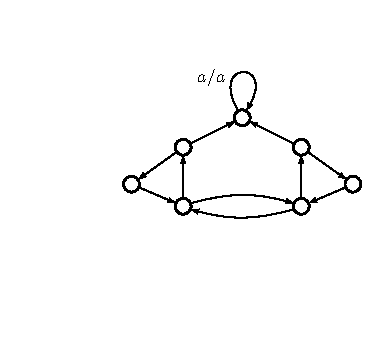
\includegraphics[scale=1.5]{../figures/bowtie}
\end{center}
\vspace{-1em}

\section*{\textsc{Knapsack} is undecidable.}

\begin{definition}
  The \defndecprob{Knapsack} problem for automaton semigroups is as
  follows: given generators $s_1\ldots s_n \in S(A)$ and some element
  $s \in S(A)$, do there exist $a_1\ldots a_n \in \N$ such
  that \[s_1^{a_1}\ldots s_n^{a_n} = s \]
\end{definition}

\begin{theorem}
  \textsc{Knapsack} is undecidable.
\end{theorem}

\begin{proofsketch}
  Reduce from Hilbert's 10 problem.
\end{proofsketch}


\section*{A monoid with undecidable \textsc{IsGroup}}

The monoid presented here serves a sort of bound; optimistically
suggesting that perhaps the class of automaton semigroups is not so
big as to have an undecidable \decprob{IsGroup}.

\begin{proofsketch}
  Reduce from the Halting problem. Given an input TM $T$, define a
  group whose generators are configurations of $T$. Set the halting
  state to the identity. If one configuration transitions to another,
  their corresponding group elements are equal.

  Then consider the submonoid generated by the start state
  $\langle s \rangle$. $\langle s \rangle$ is a group iff $T$ halts.

  In order to keep the word problem decidable, we need to modify $T$
  to be a self-verifying Turing machine.
\end{proofsketch}

\section*{Open Questions}

\begin{itemize}
\item Is \textsc{Membership} decidable in the non-abelian case?
\item Is \textsc{IsGroup} decidable in the non-abelian case?
% \item Are Markov properties decidable in automaton semigroups?
\item A wide variety of other related semigroup decision problems.
\end{itemize}

\section*{Acknowledgements}

Thanks to Klaus Sutner for guidance and Tim Becker for his continued interest.

\end{multicols}
\end{document}
